% ============================================================================
%  JobScope — Platform Update, November 2026
%  Continuation volume to JobScope_Documentation.tex (October 2026).
%  Covers the recruiter portal, CRM, Google Forms intake, roles and admin.
%
%  Compile with:  pdflatex JobScope_Update_2026-11.tex   (run twice for ToC)
%  Packages required (all standard): tikz, listings, booktabs, longtable,
%  hyperref, enumitem, geometry, xcolor, titlesec, fancyhdr.
% ============================================================================
\documentclass[11pt,a4paper]{article}

% ---- packages --------------------------------------------------------------
\usepackage[utf8]{inputenc}
\usepackage[T1]{fontenc}
\usepackage{amssymb}
\usepackage[margin=2.5cm]{geometry}
\usepackage{xcolor}
\usepackage{listings}
\usepackage{booktabs}
\usepackage{longtable}
\usepackage{enumitem}
\usepackage{tikz}
\usetikzlibrary{arrows.meta,positioning}
\usepackage{titlesec}
\usepackage{fancyhdr}

% ---- colours (defined BEFORE hyperref) --------------------------------------
\definecolor{indigo}{HTML}{4F46E5}
\definecolor{violet}{HTML}{7C3AED}
\definecolor{teal}{HTML}{0D9488}
\definecolor{codebg}{HTML}{0F172A}
\definecolor{surface}{HTML}{F1F5F9}
\definecolor{amber}{HTML}{B45309}
\definecolor{grayed}{HTML}{64748B}

\usepackage[colorlinks=true,linkcolor=indigo!75,urlcolor=teal]{hyperref}

% ---- code listing style -----------------------------------------------------
\lstset{
  basicstyle=\ttfamily\footnotesize\color{white},
  backgroundcolor=\color{codebg},
  commentstyle=\color{teal},
  keywordstyle=\color{orange!90},
  stringstyle=\color{green!70},
  numbers=left, numberstyle=\tiny\color{gray}, numbersep=6pt,
  frame=single, rulecolor=\color{gray!40}, breaklines=true,
  showstringspaces=false, aboveskip=8pt, belowskip=8pt,
}

% ---- section styling --------------------------------------------------------
\titleformat{\section}{\Large\bfseries\color{indigo}}{\thesection}{0.6em}{}
\titleformat{\subsection}{\large\bfseries\color{violet}}{\thesubsection}{0.5em}{}
\titleformat{\subsubsection}{\normalsize\bfseries\color{teal}}{\thesubsubsection}{0.5em}{}
\setlist{itemsep=2pt, topsep=4pt}

% ---- header / footer --------------------------------------------------------
\pagestyle{fancy}
\fancyhf{}
\fancyhead[L]{\small\color{grayed} JobScope --- Platform Update, November 2026}
\fancyhead[R]{\small\color{grayed} \leftmark}
\fancyfoot[C]{\small\color{grayed} \thepage}
\renewcommand{\headrulewidth}{0.4pt}

% ---- handy commands ---------------------------------------------------------
\newcommand{\file}[1]{\texttt{\small #1}}
\newcommand{\code}[1]{\texttt{#1}}
\newcommand{\tool}[1]{\texttt{#1}}
\newcommand{\api}[2]{\texttt{\small #1\,#2}}
\newcommand{\env}[1]{\texttt{\small #1}}
\newcommand{\st}[1]{{\footnotesize\bfseries\color{teal}#1}}

\setlength{\parindent}{0pt}
\setlength{\parskip}{6pt}

\begin{document}

% ============================================================================
%  TITLE PAGE
% ============================================================================
\begin{titlepage}
  \centering
  \vspace*{1.7cm}
  {\color{indigo}\rule{\textwidth}{2pt}}

  \vspace{0.8cm}
  {\fontsize{30}{36}\selectfont\bfseries\color{indigo} JobScope}\\[6pt]
  {\Large Platform Update --- November 2026}\\[2pt]
  {\large Recruiter portal, CRM, Google Forms intake, roles and admin}\\[2pt]
  {\large Continuation volume to the October 2026 technical documentation}

  \vspace{0.8cm}
  {\color{indigo}\rule{\textwidth}{2pt}}

  \vspace{1.9cm}
  \begin{minipage}{0.86\textwidth}
    \small
    \textbf{Abstract.} The October 2026 documentation described JobScope as a
    candidate-only, locally-run job-hunting assistant. Between 7 and 12
    November 2026 the repository gained a second product surface: a recruiter
    portal with its own API, a candidate CRM with resume storage and screening,
    and a Google Forms applications intake. This volume continues the
    documentation without repeating it. It records the release log since the
    last report (commits \texttt{f30145c}, \texttt{7a9e91f}, \texttt{aed44cc}),
    documents the new portal topology and role model, gives reference tables
    for every new endpoint and table, analyses the runtime JSONL logs for
    8--12 November, and lists the known gaps that remain before this can be
    called a complete ATS. Sections of the October volume that are unaffected
    (agent, scraping, filters, resume pipeline) are not restated.
  \end{minipage}

  \vfill
  {\small 13 November 2026 \\[2pt]
   Baseline: \file{docs/JobScope\_Documentation.tex}, commit \texttt{57a2a33}
   (12 October 2026)\\[2pt]
   Current head at writing: commit \texttt{aed44cc} (12 November 2026)\\[2pt]
   Build target: Python 3.14, Windows / PowerShell \\[2pt]
   File: \file{docs/JobScope\_Update\_2026-11.tex}}
\end{titlepage}

\tableofcontents
\clearpage

% ============================================================================
\section{Scope and Release Log}
\label{u:scope}

\subsection{Baseline and reading order}
The previous volume, \file{JobScope\_Documentation.tex}, remains authoritative
for installation, the LangGraph agent, board scraping, Gmail fallback, the
resume/BM25 pipeline, ATS scoring, the original candidate API, and the
seven-step tutorial. This volume supersedes it only where the platform changed:
authentication and the data model, the route surface, the front-end pages, the
test inventory, and operations/log analysis. Read the October volume first,
then this one.

\subsection{Commits since the last report}
\begin{center}
\begin{tabular}{@{}lllp{7.4cm}@{}}
\toprule
\textbf{Commit} & \textbf{Date} & \textbf{Message} & \textbf{Scope}\\
\midrule
\texttt{57a2a33} & 12 Oct & documentation updated & Baseline: October documentation\\
\texttt{f30145c} & 7 Nov & Update JobScope project &
  Portal split: \file{home.html}, \file{admin.html}, recruiter shell,
  \file{dashboard.py} routes, auth schema expansion\\
\texttt{7a9e91f} & 8 Nov & updates on recuriter portal &
  \file{crm.py}, \file{recruiter\_api.py}, expanded \file{auth.py},
  \file{recruiter.html} workspace\\
\texttt{aed44cc} & 12 Nov & few fixes &
  \file{candidates\_api.py}, \file{google\_forms\_api.py}, new tests,
  README and requirements\\
\bottomrule
\end{tabular}
\end{center}

The apparent 350k-line deletion in the raw diff is the removal of the
unrelated \file{crawl4ai-main/} reference checkout, not application code. The
application diff is roughly 10.5k inserted lines and a few hundred changed
lines.

\subsection{New features at a glance}
\begin{center}
\begin{tabular}{@{}llp{8.1cm}@{}}
\toprule
\textbf{ID} & \textbf{State} & \textbf{Feature}\\
\midrule
F1 & \st{stable} & Role model: \code{candidate}, \code{recruiter},
     \code{super\_admin}; first account is owner\\
F2 & \st{stable} & Recruiter portal SPA at \file{/recruiter} with jobs,
     applications, candidates, pipeline, interviews, calendar and tasks\\
F3 & \st{stable} & \file{recruiter\_api.py}: company-scoped recruiter API,
     including candidate-proposed interview slots\\
F4 & \st{stable} & Candidate CRM phase 1: resume upload/download, notes,
     tags, sourced pipeline, resume screening\\
F5 & \st{stable} & Google Forms applications: per-recruiter OAuth, form
     linking, response sync, Drive CV import\\
F6 & \st{stable} & Super-admin portal and user CRUD at \file{/admin}\\
F7 & \st{partial} & \file{crm.py}: 19-stage CRM/ATS data layer, committed but
     not mounted in \file{dashboard.py}\\
F8 & \st{stable} & SQLite schema expansion: companies, jobs, applications,
     interviews, offers, placements, tasks, audit and more\\
F9 & \st{stable} & New test modules for the recruiter loop, candidates and
     Google Forms (33 tests passing on 13 November)\\
F10 & \st{stable} & Operational delta: new Google dependencies, one new
     environment variable, new storage directories, log analysis\\
\bottomrule
\end{tabular}
\end{center}

State labels: \st{stable} means routed and tested; \st{partial} means the code
exists but has no HTTP surface yet; \st{planned} is used later for navigation
entries that are visibly marked ``soon'' in the UI.

% ============================================================================
\section{Portal Topology and Role Model}
\label{u:portals}

\subsection{Page routes}
\begin{center}
\begin{tabular}{@{}lp{3.8cm}p{8.2cm}@{}}
\toprule
\textbf{Path} & \textbf{File} & \textbf{Behaviour}\\
\midrule
\file{/} & \file{static/index.html} &
  Candidate workspace. Its own gate offers a candidate/recruiter toggle; a
  signed-in recruiter or super admin is redirected to \file{/recruiter}.\\
\file{/candidate} & \file{static/index.html} &
  Same candidate workspace under an explicit path.\\
\file{/recruiter} & \file{static/recruiter.html} &
  Recruiter CRM workspace. Falls back to \file{index.html} if the file is
  missing.\\
\file{/admin} & \file{static/admin.html} &
  Super-admin account manager. The HTML is public; every data call behind it
  is guarded.\\
\file{/health} & --- & Liveness probe: \code{\{"status": "healthy"\}}.\\
404 (non-API) & \file{static/404.html} &
  HTML error page; \file{/api/} and \file{/static/} keep JSON.\\
\bottomrule
\end{tabular}
\end{center}

Two routing details matter for maintainers:
\begin{itemize}[leftmargin=2em]
  \item \file{static/home.html} (a standalone candidate/recruiter sign-in
        page) ships in the repository but no FastAPI route serves it in this
        build. It is currently dead weight; \file{/} serves
        \file{index.html}, whose gate already has the portal toggle. Either
        mount it at \file{/home} or delete it, but do not document it as a
        working entry point.
  \item The 404 handler distinguishes a mistyped page from a mistyped API
        call. That keeps browser navigation human-readable without breaking
        clients that expect JSON errors.
\end{itemize}

\subsection{Roles}
\begin{center}
\begin{tabular}{@{}lp{11.4cm}@{}}
\toprule
\textbf{Role} & \textbf{Meaning and rights}\\
\midrule
\code{candidate} & Default role. Uses the agent, resumes and applications.
  Can read published jobs and apply.\\
\code{recruiter} & Uses the recruiter portal. Company-scoped: jobs,
  applications, candidates, tasks, interviews and screening are filtered by
  the recruiter's \code{company\_id}.\\
\code{super\_admin} & Full recruiter rights plus \api{/api/admin/*} user
  management. The first registered account is also marked
  \code{is\_owner}, and ownership is accepted by the admin guard.\\
fixed admin & A legacy, separate login at \file{/admin} with its own
  \code{js\_admin\_session} cookie. It is not a row in \code{users}.\\
\bottomrule
\end{tabular}
\end{center}

Registration accepts only \code{candidate} or \code{recruiter}; anything else
is coerced to \code{candidate}. The admin API may create
\code{candidate}, \code{recruiter} or \code{super\_admin}. Note that the
inline comment on \code{users.role} in \file{auth.py} still says
``candidate or recruiter''; the executable guard accepts
\code{super\_admin} as well. Treat the code as the source of truth and fix the
comment.

\subsection{Sign-in, registration and verification}
\begin{itemize}[leftmargin=2em]
  \item The login endpoint ignores the optional \code{role} field. The stored
        account role decides where the browser goes: candidate data stays in
        \file{index.html}; recruiter and super-admin accounts are redirected to
        \file{/recruiter}. The candidate/recruiter toggle on the gate is a
        visual affordance, not an authorisation check.
  \item Unknown address and wrong password return the same 401 message, so
        login cannot be used to enumerate accounts. Failures are logged as
        \code{login\_failed}.
  \item The first account becomes owner and adopts any legacy
        \file{profiles.json} CV sessions. With SMTP configured, verification
        mail is sent and the account stays limited until the link is followed;
        without SMTP the link is returned to the page and the account is
        marked verified so a fresh checkout remains usable.
  \item Password reset invalidates every session for that account. Sessions
        remain HTTP-only, SameSite=Lax, 25-minute idle with a five-minute
        extension, and a 30-day absolute cap.
\end{itemize}

\subsection{Portal diagram}
\begin{center}
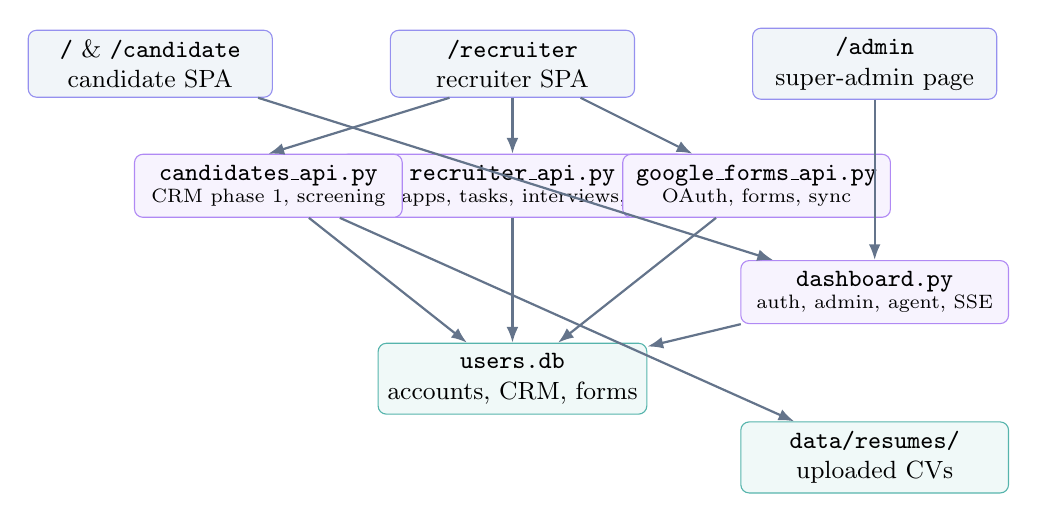
\begin{tikzpicture}[
  box/.style={draw=indigo!60, fill=surface, rounded corners=3pt,
              align=center, font=\small, minimum width=3.1cm,
              minimum height=0.85cm},
  api/.style={draw=violet!60, fill=violet!6, rounded corners=3pt,
              align=center, font=\scriptsize, minimum width=3.4cm,
              minimum height=0.8cm},
  db/.style={draw=teal!70, fill=teal!6, rounded corners=3pt,
             align=center, font=\small, minimum width=3.4cm,
             minimum height=0.9cm},
  ar/.style={-{Latex[length=2mm]}, draw=grayed, thick}
]
\node[box] (idx) at (0,3.1) {\file{/} \& \file{/candidate}\\candidate SPA};
\node[box] (rec) at (4.6,3.1) {\file{/recruiter}\\recruiter SPA};
\node[box] (adm) at (9.2,3.1) {\file{/admin}\\super-admin page};

\node[api] (ra) at (4.6,1.55) {\file{recruiter\_api.py}\\
  jobs, apps, tasks, interviews, slots};
\node[api] (ca) at (1.5,1.55) {\file{candidates\_api.py}\\
  CRM phase 1, screening};
\node[api] (ga) at (7.7,1.55) {\file{google\_forms\_api.py}\\
  OAuth, forms, sync};
\node[api] (da) at (9.2,0.2) {\file{dashboard.py}\\
  auth, admin, agent, SSE};

\node[db] (udb) at (4.6,-0.9) {\file{users.db}\\accounts, CRM, forms};
\node[db] (fs) at (9.2,-1.9) {\file{data/resumes/}\\uploaded CVs};

\draw[ar] (idx) -- (da);
\draw[ar] (rec) -- (ra);
\draw[ar] (rec.south) ++(-0.8,0) -- (ca.north);
\draw[ar] (rec) -- (ga);
\draw[ar] (adm) -- (da);
\draw[ar] (ra) -- (udb);
\draw[ar] (ca) -- (udb);
\draw[ar] (ga) -- (udb);
\draw[ar] (ca) -- (fs);
\draw[ar] (da) -- (udb);
\end{tikzpicture}
\end{center}

The three new routers are included immediately after
\code{app = FastAPI(...)} and before every older route in
\file{dashboard.py}. FastAPI matches the first registered route, so this order
is deliberate: the newer, validated recruiter/candidate handlers win over the
older same-path stubs.

% ============================================================================
\section{Recruiter Portal (\file{static/recruiter.html})}
\label{u:rec-ui}

The recruiter portal is a single-file SPA (about 1{,}700 lines) with no build
step, matching the candidate front end. It is served verbatim and talks to the
same-origin JSON API with the existing \code{js\_session} cookie.

\subsection{Navigation}
\begin{center}
\begin{tabular}{@{}llp{7.8cm}@{}}
\toprule
\textbf{Group} & \textbf{Page} & \textbf{State}\\
\midrule
Workspace & Overview, My Tasks, Calendar & Implemented\\
Talent management & Candidates & Implemented\\
 & Talent Pool, Saved Candidates & Navigation marked ``soon''\\
Recruitment & Jobs, Applications, Google Forms & Implemented\\
 & Recruitment Pipeline, Interviews & Implemented\\
 & Offers & Navigation marked ``soon'' (API not mounted)\\
AI recruitment & Resume Screening & Implemented\\
 & AI Candidate Search, Candidate Matching & Navigation marked ``soon''\\
Reports & Recruitment Analytics & Navigation marked ``soon''\\
Administration & User Management & Visible to super admins only\\
Settings & Company Profile, Recruiter Profile, Account Settings &
  Implemented\\
 & Team Management & Navigation marked ``soon''\\
\bottomrule
\end{tabular}
\end{center}

\subsection{What each page does}
\begin{itemize}[leftmargin=2em]
  \item \textbf{Overview.} Reads \api{GET}{/api/recruiter/dashboard/stats}
        and renders counters (jobs, applications, shortlisted, interviews,
        offers, hires, candidates, pending slots) plus recent applications and
        jobs.
  \item \textbf{Jobs.} Lists company jobs, creates and edits them, and moves
        them through \code{draft}, \code{published}, \code{paused} and
        \code{closed}. Creating a job while Google is connected also creates
        and links an application form; the response carries
        \code{form: \{form\_id, form\_title, responder\_uri\}} or \code{null}.
  \item \textbf{Applications.} Filters company applications, opens the Q\&A
        transcript for Google Forms applications, changes status, and
        schedules interviews with the candidate's own email address.
  \item \textbf{Candidates.} Adds, edits and deletes recruiter-owned
        candidates; the drawer shows notes, tags, the active resume with
        extracted skills, and sourced pipeline rows. Resume upload accepts PDF
        or DOCX up to 5\,MB.
  \item \textbf{Recruitment Pipeline.} Renders sourced
        \code{pipeline\_entries} for the caller's company and moves entries
        across the application-stage whitelist.
  \item \textbf{Resume Screening.} Scores every company candidate resume
        against one job through the existing \file{ats\_score.py} code. There
        is no second matching implementation in the page.
  \item \textbf{Interviews \& Calendar.} Lists interviews, schedules new
        ones, shows candidate-proposed slots, and confirms or declines a slot.
        Own calendar events are separate from interviews.
  \item \textbf{My Tasks.} Per-recruiter tasks with status and priority;
        completed/cancelled items sort last.
  \item \textbf{Company / Recruiter Profile / Settings.} Company identity,
        recruiter title and phone, and account preferences. A recruiter
        cannot create a job until a company is set up.
\end{itemize}

The portal deliberately reuses plain forms and fetch calls. There is no
framework, bundler or generated client, so the only contract between front end
and back end is the JSON shape documented in the next section. The theme
toggle, keyboard focus styles and modal/drawer behaviour are local to the
file.

% ============================================================================
\section{Recruiter API (\file{recruiter\_api.py})}
\label{u:rec-api}

\subsection{Guards and tenancy}
Every route depends on one of three helpers:
\code{\_user} (any signed-in account), \code{\_recruiter}
(\code{recruiter} or \code{super\_admin}), and \code{\_candidate}
(\code{candidate} or \code{super\_admin}). A recruiter with no
\code{recruiter\_profiles.company\_id} gets \code{400}
``Set up your company first'' on write routes and empty lists on read routes.

Tenancy is enforced with company joins, not with a separate permission table.
A job, application, interview, slot or link that belongs to another company is
reported as \code{404}, never \code{403}, so the API does not confirm that the
record exists. Several tests assert exactly this.

\subsection{Endpoint reference}
\begin{longtable}{@{}p{1.35cm}p{6.15cm}p{7.6cm}@{}}
\toprule
\textbf{Method} & \textbf{Path} & \textbf{Purpose}\\
\midrule
\endhead
GET & \api{/api/recruiter/company} & Company profile for the caller.\\
POST & \api{/api/recruiter/company} & Create or update the company.\\
GET & \api{/api/recruiter/profile} & Recruiter identity (name, title, phone,
      company).\\
POST & \api{/api/recruiter/profile} & Update that identity.\\
GET & \api{/api/recruiter/jobs} & Company jobs, optional \code{status}.\\
POST & \api{/api/recruiter/jobs} & Create a job; optionally creates a Google
      Form and links it.\\
POST & \api{/api/recruiter/jobs/\{job\_id\}/update} & Patch job fields.\\
POST & \api{/api/recruiter/jobs/\{job\_id\}/status} & Draft / publish / pause /
      close.\\
GET & \api{/api/recruiter/applications} & Company applications, optional
      \code{job\_id}.\\
POST & \api{/api/recruiter/applications/\{app\_id\}/status} & Move an
      application within the status whitelist.\\
GET & \api{/api/recruiter/dashboard/stats} & Counters and recent activity.\\
GET & \api{/api/recruiter/tasks} & Caller's tasks, unfinished first.\\
POST & \api{/api/recruiter/tasks} & Create a task.\\
POST & \api{/api/recruiter/tasks/\{task\_id\}/update} & Patch a task.\\
DELETE & \api{/api/recruiter/tasks/\{task\_id\}} & Delete a task.\\
GET & \api{/api/recruiter/interviews} & Company interviews with candidate and
      job labels.\\
POST & \api{/api/recruiter/interviews} & Book an interview; returns
      \code{mail: \{sent, error\}}.\\
POST & \api{/api/recruiter/interviews/\{id\}/update} & Reschedule or change
      status.\\
GET & \api{/api/recruiter/calendar} & Own events, proposed slots and
      interviews.\\
POST & \api{/api/recruiter/events} & Create a personal calendar event.\\
DELETE & \api{/api/recruiter/events/\{id\}} & Delete an own event.\\
POST & \api{/api/recruiter/slots/\{id\}/confirm} & Accept a candidate slot,
      book the interview and decline the sibling slots.\\
POST & \api{/api/recruiter/slots/\{id\}/decline} & Decline one proposed slot.\\
GET & \api{/api/candidate/applications} & Candidate's applications, slots and
      next interview.\\
POST & \api{/api/candidate/applications/\{id\}/slots} & Offer 1--10 future
      slots (15--480 minutes each).\\
DELETE & \api{/api/candidate/slots/\{id\}} & Withdraw a still-proposed slot.\\
\bottomrule
\end{longtable}

The module also declares \api{GET/POST/DELETE}{/api/candidates} for
recruiter-owned candidate records. Those handlers are shadowed by
\file{candidates\_api.py} because that router is registered first. Keep them
only as compatibility fallback, or delete them to remove the duplicate surface.

\subsection{Interview slots}
Slot handling is a small state machine:
\begin{center}
\code{proposed} $\rightarrow$ \code{booked} on recruiter confirmation, or
\code{proposed} $\rightarrow$ \code{declined} on refusal. A candidate may
delete a slot only while it is still \code{proposed}; a booked slot is
history.
\end{center}
Confirming one slot sets every other proposed slot on the same application to
\code{declined} in the same transaction, then books the interview. This is the
only place that can flip several slots at once, so the ``one confirmed
interview per application'' rule cannot be bypassed by the UI.

\subsection{Time and mail contract}
Times cross the wire as UTC ISO strings ending in \code{Z}; the browser sends
and renders them in the viewer's time zone. The server normalises
\code{\_iso()} input. Interview e-mail is sent with the job title, UTC time,
duration, meeting link/location and instructions. Delivery is reported in
\code{mail} and never rolls back a booking: a failed SMTP call leaves the
interview scheduled and the candidate visible in Applications. For a Google
Forms respondent, the address and name are exactly the ones collected by the
form.

\subsection{Module-created tables}
\file{recruiter\_api.py} creates its own tables lazily on first use:
\code{calendar\_events} and \code{interview\_slots}. It uses the core
\code{companies}, \code{jobs}, \code{applications}, \code{interviews} and
\code{tasks} tables from \file{auth.SCHEMA}. The lazy creation is keyed by
\code{auth.DB\_FILE}, so a test that redirects the database also gets a fresh
schema.

% ============================================================================
\section{Candidate CRM, Phase 1 (\file{candidates\_api.py})}
\label{u:cand}

\subsection{Two kinds of candidate}
The CRM keeps a master candidate in \file{auth.py}'s legacy \code{candidates}
table (per recruiter, with an email and status) and a job application in
\code{applications} (per company and job). Pipeline stage lives on the
application, so one person can be screening for one job and interviewing for
another. Candidate records are owned by the recruiter who added them:
\code{GET /api/candidates} filters on \code{candidates.user\_id}, while sourced
pipeline entries are company-scoped through \code{recruiter\_profiles}.
Another company's candidate or pipeline entry returns \code{404}.

\subsection{Resume pipeline}
Upload is deliberately narrow and validated at the trust boundary:
\begin{itemize}[leftmargin=2em]
  \item PDF or DOCX, at most 5\,MB, validated by file signature rather than
        by the client-supplied name.
  \item Text is extracted with the existing CV helpers. Image-only PDFs fall
        back to the Tier-2 OCR path (\file{cv\_ocr.py}), the same one used by
        the candidate workspace.
  \item One active resume per candidate: a successful upload deletes the
        previous row and file only after the new row is written. A failed
        write removes the new file and leaves the old record intact.
  \item Files are stored outside the static tree in \file{data/resumes/} with
        a random stored name; download is an authenticated route with
        \code{Content-Disposition: attachment}. A stored file can never be
        fetched by URL guessing.
  \item Skills are extracted from the text with \file{resume\_data.py};
        screening searches the parsed text, so a skill filter matches the CV
        body, not just the tags.
\end{itemize}

\subsection{Notes, tags and sourced candidates}
Notes are free text up to 5{,}000 characters, recording the author display
name and a UTC timestamp; they are listed newest first. Tags are per
(candidate, tag) pairs up to 60 characters, added idempotently and removable
one at a time. Sourced pipeline entries are created with
\code{\{job\_id, candidate\_id, status?\}}, unique per
\code{(company, job, candidate)}; repeating the call updates the existing entry
instead of duplicating it. A sourced candidate may have no user account.

\subsection{Resume screening}
\api{GET}{/api/recruiter/screening?job\_id=} scores every company candidate
resume against one job using \code{ats\_score.score\_resume}. It returns the
ATS total, band, matched keywords, missing keywords, and best-first ordering.
The route never re-implements matching; it is the same scorer used by the
resume generator and \code{/api/screen}. A job from another company returns
\code{404}.

\subsection{Endpoint reference}
\begin{longtable}{@{}p{1.35cm}p{6.3cm}p{7.45cm}@{}}
\toprule
\textbf{Method} & \textbf{Path} & \textbf{Purpose}\\
\midrule
\endhead
GET & \api{/api/candidates} & Filter own candidates by \code{q},
      \code{skill}, \code{status}, \code{tag}, \code{limit}, \code{offset}.\\
GET & \api{/api/candidates/\{id\}} & Detail, notes, tags, active resume and
      sourced pipeline rows.\\
POST & \api{/api/candidates} & Create or update a candidate record.\\
DELETE & \api{/api/candidates/\{id\}} & Cascade delete notes, tags, resume row,
      stored file and sourced company entries.\\
POST & \api{/api/candidates/\{id\}/notes} & Add a note.\\
POST & \api{/api/candidates/\{id\}/tags} & Add or remove one tag.\\
POST & \api{/api/candidates/\{id\}/resume} & Multipart upload; replaces the
      active resume.\\
GET & \api{/api/candidates/\{id\}/resume} & Authenticated attachment download.\\
GET & \api{/api/recruiter/pipeline} & Company sourced pipeline rows.\\
POST & \api{/api/recruiter/pipeline} & Hand-add a candidate to a job.\\
POST & \api{/api/recruiter/pipeline/\{id\}/status} & Move a sourced entry.\\
GET & \api{/api/recruiter/screening} & ATS score of company resumes against a
      job.\\
\bottomrule
\end{longtable}

\subsection{Module-created tables}
\code{candidate\_resumes} (one active row per candidate), \code{candidate\_tags},
\code{candidate\_notes} and \code{pipeline\_entries}. The first three are
keyed by recruiter \code{user\_id}; \code{pipeline\_entries} is keyed by
company, job and candidate. The cascading delete in the API is intentional:
deleting a candidate removes the stored CV and sourced entries, which is what
the UI's confirmation text promises.

% ============================================================================
\section{Google Forms Applications (\file{google\_forms\_api.py})}
\label{u:gforms}

\subsection{Product model}
A candidate can apply through a Google Form instead of the portal. Each
recruiter connects their own Google account, links a form to one of their jobs,
and syncs responses. Every response becomes a normal \code{applications} row
with \code{source = 'google\_form'}, so it appears in Applications, Resume
Screening and the pipeline like any other application. Answers are preserved
as a Q\&A transcript in \code{applications.cover\_letter} (capped at 4{,}000
characters).

The integration is optional at import time: the Google libraries are imported
lazily, so a checkout without them still starts and the portal reports the
integration as unavailable rather than failing to boot.

\subsection{OAuth lifecycle}
\begin{itemize}[leftmargin=2em]
  \item Scopes: \code{openid}, \code{userinfo.email},
        \code{forms.responses.readonly}, \code{forms.body} and
        \code{drive.readonly}. Forms body is needed to create and publish
        application forms; Drive read-only downloads uploaded CVs.
  \item The OAuth client is the existing installed-app
        \file{client\_secret.json} (\env{GOOGLE\_OAUTH\_CREDENTIALS}), shared
        with the Gmail tools. Only the Forms and Drive APIs need to be enabled
        in that project.
  \item Consent uses a single-use \code{state}, a PKCE verifier and the exact
        redirect URI, stored together with a 10-minute TTL. The callback
        replays all three. This is why a callback on a different host or port
        can still finish, and why an older state cannot be replayed.
  \item The refresh token is stored per recruiter in \code{google\_oauth};
        revoking one recruiter's access cannot affect another's.
  \item Token exchange talks to Google's token endpoint directly so a refusal
        surfaces Google's own code (for example \code{invalid\_grant}) instead
        of a generic failure.
  \item \env{GOOGLE\_FORMS\_REDIRECT\_URI} is optional. When unset, the URI
        is derived from the host and port serving the portal, so both
        \code{localhost} and \code{127.0.0.1} work. If set, it must be listed
        verbatim under the OAuth client's authorised redirect URIs.
\end{itemize}

\subsection{Form creation and linking}
\api{POST}{/api/recruiter/jobs} calls \code{create\_form\_for\_job()} after the
job is created. The function creates a published form in the recruiter's own
Drive with four questions: name (required), email (required), phone, and
``Why do you want this role?''. The form is linked to the job in
\code{google\_form\_links}. If the recruiter has not connected Google, or
Google fails, job creation still succeeds and the response carries
\code{form: null}. This keeps the optional integration from becoming a
dependency of the core write path.

Forms can also be linked by URL or id. \code{\_form\_id()} accepts an edit
link, a responder link or a bare id (tested); a responder link is rejected with
a usable hint.

\subsection{Sync semantics}
\api{POST}{/api/recruiter/integrations/google-forms/links/\{id\}/sync} pulls
all responses and returns:
\begin{center}
\code{\{added, seen, skipped, duplicates, no\_email, resumes\}}.
\end{center}
\begin{center}
\begin{tabular}{@{}llp{9.3cm}@{}}
\toprule
\textbf{Field} & \textbf{Meaning} & \textbf{Notes}\\
\midrule
\code{seen} & responses read & Includes duplicates and unusable rows.\\
\code{added} & new applications & Inserted with \code{ON CONFLICT DO NOTHING}
  on \code{(job\_id, candidate\_user\_id)}.\\
\code{duplicates} & already imported & Re-sync never rewrites the recruiter's
  status.\\
\code{no\_email} & skipped & No address anywhere in the response; the app never
  invents one.\\
\code{resumes} & CVs imported & Each downloaded from the respondent's Drive
  into \file{data/resumes/}.\\
\bottomrule
\end{tabular}
\end{center}

A response with no usable email is skipped rather than turned into an account.
A form that never asks for an address imports nothing; enable
\emph{Settings $\rightarrow$ Responses $\rightarrow$ Collect email addresses}
or add an Email question. A failed CV download keeps the application and is
simply not counted in \code{resumes}; the API does not roll back a good
application because one attachment was unreadable.

\subsection{Respondent accounts and claiming}
Each respondent gets an unverified candidate account keyed by their normalised
email. The stored password hash is prefixed with \code{!} and random, so it
can never match a password. When that person later signs up or resets the
password with the same address, they claim the existing row and inherit the
application history. A respondent who never signs up remains a valid
company-visible candidate.

\subsection{Google Forms endpoint reference}
\begin{longtable}{@{}p{1.35cm}p{6.6cm}p{7.15cm}@{}}
\toprule
\textbf{Method} & \textbf{Path} & \textbf{Purpose}\\
\midrule
\endhead
GET & \api{/api/recruiter/integrations/google-forms} & Connection state,
      connected address and linked forms.\\
GET & \api{/api/recruiter/integrations/google-forms/start} & Build the consent
      URL; store state, PKCE verifier and redirect URI.\\
GET & \api{/api/recruiter/integrations/google-forms/callback} & Exchange the
      code, store the refresh token, return to
      \file{/recruiter\#google-forms}.\\
DELETE & \api{/api/recruiter/integrations/google-forms} & Forget the token;
      linked forms remain but syncs stop.\\
POST & \api{/api/recruiter/integrations/google-forms/links} & Link a form
      (URL or id) to an own job.\\
DELETE & \api{/api/recruiter/integrations/google-forms/links/\{id\}} & Unlink;
      another company's link returns 404.\\
POST & \api{/api/recruiter/integrations/google-forms/links/\{id\}/sync} &
      Import responses and uploaded CVs.\\
\bottomrule
\end{longtable}

\subsection{Setup checklist}
\begin{enumerate}[leftmargin=2em]
  \item Enable the Google Forms API and Google Drive API in the same Google
        Cloud project as \file{client\_secret.json}.
  \item Add the callback URL as an authorised redirect URI, or leave
        \env{GOOGLE\_FORMS\_REDIRECT\_URI} unset and use the derived one.
  \item Open \emph{Google Forms} in the recruiter portal and choose
        \emph{Connect Google}.
  \item Link an existing form, or let job creation make one.
  \item If CVs matter, add one \textbf{File upload} question to the form in the
        Google Forms UI once. The Forms API cannot create that question type.
\end{enumerate}

That last point is a deliberate, documented shortcut:
\code{shortcut: the Forms API cannot create file-upload questions, add one once by hand; upgrade when Google exposes it.}

% ============================================================================
\section{CRM/ATS Data Layer (\file{crm.py})}
\label{u:crm}

\file{crm.py} is a pure data layer for a fuller ATS than the current routes
expose. It imports only \file{auth.py} and assumes an authorised caller; the
API layer is responsible for permissions. It is \emph{not} imported by
\file{dashboard.py} in this build, so none of its functions are reachable over
HTTP yet. Treat it as phase-2 groundwork, not a shipped feature.

\subsection{The nineteen-stage pipeline}
The module centralises the pipeline vocabulary so a Kanban board, filters and
closure maths cannot drift apart:
\begin{center}
\begin{tabular}{@{}lll@{}}
\toprule
\textbf{Stage} & \textbf{Stage} & \textbf{Stage}\\
\midrule
sourced & screening\_pending & screening\_completed\\
shortlisted & submitted\_to\_client & client\_review\\
interview\_scheduled & interview\_in\_progress & interview\_completed\\
selected & offer\_negotiation & offer\_released\\
offer\_accepted & notice\_period & joined\\
placed & rejected & withdrawn\\
on\_hold & & \\
\bottomrule
\end{tabular}
\end{center}
Active stages exclude \code{rejected}, \code{withdrawn} and \code{placed}.
Old \code{applications.status} values are still written from a stage move so
the candidate portal keeps working; for example \code{joined} maps to
\code{hired} and \code{on\_hold} maps to \code{on\_hold}.

\subsection{Modules in the file}
\begin{center}
\begin{tabular}{@{}lp{11cm}@{}}
\toprule
\textbf{Area} & \textbf{Functions}\\
\midrule
Candidates & list, get, save, archive, portfolio, documents, experience,
  education, skills, notes, communications\\
Companies & list, get, save, delete, contacts\\
Jobs & list, get, save, cancel, closure maths\\
Applications & list, get, add candidate, move stage, stage history\\
Interviews & list, get, save, feedback\\
Offers & list, get, save, status transitions, history\\
Placements & list, get, save, status, synchronisation into application and
  job closure\\
Tasks & list, save, status, delete\\
Activity & audit log, activity feed, notifications, notification read state\\
Reporting & dashboard counters, recruiter performance, analytics, global
  search, CSV export\\
\bottomrule
\end{tabular}
\end{center}

\subsection{Invariants worth preserving}
\begin{itemize}[leftmargin=2em]
  \item A job is cancelled rather than deleted, because applications and
        placements are history.
  \item A placement propagates into the application stage and the job closure
        in one transaction; a partial placement update would make two screens
        disagree.
  \item Every stage move writes \code{application\_stage\_history} and an
        audit row, so the pipeline can be reconstructed later.
  \item Uploads go to \file{uploads/} outside the static tree, are capped at
        10\,MB, and are restricted to PDF, Office, text and image extensions.
  \item Dates are UTC ISO strings, except where a dashboard counter needs
        arithmetic days; conversion stays in the data layer.
\end{itemize}

The missing HTTP surface is the main gap: offers, placements, talent pools,
analytics and global search already have data functions but no validated
endpoints, which is why the recruiter navigation marks several of them
``soon''.

% ============================================================================
\section{Authentication, Administration and Risk}
\label{u:auth}

\subsection{Schema additions}
\code{users} gained \code{role} (default \code{candidate}),
\code{nickname} and \code{avatar}. New tables under \file{auth.SCHEMA}:
\begin{center}
\begin{tabular}{@{}llp{8.5cm}@{}}
\toprule
\textbf{Group} & \textbf{Tables} & \textbf{Purpose}\\
\midrule
Identity & \code{recruiter\_profiles}, \code{candidate\_profiles} &
  Company link, title/phone; full candidate master profile\\
Company & \code{companies}, \code{company\_contacts} &
  Employer record and client contacts\\
Jobs & \code{jobs}, \code{job\_assignments} &
  Postings, requirements, recruiter assignment\\
Pipeline & \code{applications}, \code{application\_stage\_history},
  \code{talent\_pools}, \code{talent\_pool\_members} &
  Applications, immutable stage history, pools\\
Interviews & \code{interviews}, \code{interview\_feedback} &
  Scheduling and structured feedback\\
Offers & \code{offers}, \code{offer\_history}, \code{placements} &
  Offer lifecycle and placement record\\
Work & \code{tasks}, \code{notifications}, \code{activities},
  \code{audit\_logs} & Reminders, inbox, activity feed, audit trail\\
Documents & \code{recruiter\_notes}, \code{communications},
  \code{candidate\_documents}, \code{candidate\_experiences},
  \code{candidate\_education}, \code{candidate\_skills} &
  Notes, call/mail log, CV and profile sub-records\\
\bottomrule
\end{tabular}
\end{center}

\subsection{Migrations}
\file{auth.py} keeps an additive \code{\_migrate()} list because
\code{CREATE TABLE IF NOT EXISTS} cannot add a column to an existing table.
Each entry is checked against \code{PRAGMA table\_info} and added only when
missing. No column is dropped or retyped. This is how an existing
\code{users.db} gains \code{role}, the CRM fields and
\code{applications.stage/source}. The same policy must continue: a destructive
migration would erase real accounts and applications.

\subsection{Admin surface}
\api{GET}{/api/admin/users} lists accounts; \api{POST}{/api/admin/users}
creates one and marks it verified; \api{POST}{/api/admin/users/\{id\}/update}
changes email, password, role or owner flag; \api{DELETE}{/api/admin/users/\{id\}}
deletes one. A password change also deletes every session for that user. A
super admin cannot delete their own account. The admin guard accepts either
the fixed admin cookie or a signed-in \code{super\_admin}/\code{is\_owner}
account.

\begin{center}
\begin{tabular}{@{}p{1.6cm}p{5.9cm}p{7.1cm}@{}}
\toprule
\textbf{Method} & \textbf{Path} & \textbf{Purpose}\\
\midrule
POST & \api{/api/admin/login} & Fixed-admin login, sets \code{js\_admin\_session}\\
POST & \api{/api/admin/logout} & Clears that cookie\\
GET & \api{/api/admin/session} & Reports fixed-admin state\\
GET & \api{/api/admin/users} & List accounts\\
POST & \api{/api/admin/users} & Create account with role\\
POST & \api{/api/admin/users/\{id\}/update} & Email, password, role, owner\\
DELETE & \api{/api/admin/users/\{id\}} & Delete account\\
\bottomrule
\end{tabular}
\end{center}

\subsection{Security findings that must not be ignored}
\begin{enumerate}[leftmargin=2em]
  \item \textbf{Hard-coded fixed-admin credentials.} \file{dashboard.py}
        defines the fallback admin username and password as string literals
        and derives a cookie token from them. Anyone who can read the source
        can sign into \file{/admin} on any deployment that has not changed
        them. Move this to an environment secret, hash it, and add a startup
        refusal when the default is still in use. This is the highest-priority
        fix before exposing the app beyond localhost.
  \item \textbf{The fixed-admin cookie never expires} and is a deterministic
        hash, not a random session token. It cannot be revoked server-side
        without changing the password literal.
  \item \textbf{The admin HTML page is public.} Only its data APIs are guarded.
        That is acceptable for a local tool, but a public deployment should
        gate the page too.
  \item \textbf{No CSRF token.} State-changing endpoints rely on
        SameSite=Lax and same-origin fetch. Keep the app on
        \code{127.0.0.1} or behind TLS and a trusted proxy; do not embed it in
        a third-party site.
  \item \textbf{Two application vocabularies coexist.} The legacy
        \code{applications.status} (15 values), the CRM 19-stage vocabulary and
        the recruiter API whitelist must be kept in sync by the mapping in
        \file{crm.py}. A status added to one without the others will silently
        disappear from a filter.
  \item \textbf{Dead or shadowed surfaces.} \code{candidates} handlers in
        \file{recruiter\_api.py} are shadowed by \file{candidates\_api.py};
        \file{static/home.html} is unreachable; parts of the short-lived route
        history remain in \file{dashboard.py}. Delete rather than extend them.
\end{enumerate}

% ============================================================================
\section{Tests and Verification}
\label{u:tests}

\subsection{New test modules}
\begin{center}
\begin{tabular}{@{}lrl@{}}
\toprule
\textbf{Module} & \textbf{Tests} & \textbf{What it covers}\\
\midrule
\file{tests/test\_recruiter\_loop.py} & 1 &
  End-to-end hiring loop: job, application, interview, calendar slot\\
\file{tests/test\_candidates.py} & 9 &
  Candidate round trip, DOCX replace, OCR fallback, ATS screening, bad input,
  role guards, cross-company 404, cascading delete\\
\file{tests/test\_google\_forms.py} & 21 &
  OAuth start/callback/PKCE/state replay, sync, no-email skip, Drive CV
  import, failed download, interview mail, form creation, company scoping,
  disconnect, account claiming, role guards, form-id parsing\\
\file{tests/test\_auth.py} & 43 &
  Accounts, roles, sessions, tokens and identity (expanded)\\
\file{tests/test\_auth\_routes.py} & 62 &
  HTTP auth surface (expanded)\\
\file{tests/test\_dashboard.py} & 155 &
  Existing dashboard surface, including the new portal assertions\\
\bottomrule
\end{tabular}
\end{center}

The three new modules were executed on 13 November 2026:

\begin{lstlisting}[language=bash]
.\.venv\Scripts\python.exe -m pytest `
  tests/test_candidates.py tests/test_google_forms.py `
  tests/test_recruiter_loop.py -q
# 33 passed
\end{lstlisting}

The suite's autouse fixture redirects \file{users.db} and
\file{profiles.json} to a temporary directory, so these tests do not touch
real accounts. There is no direct test module for \file{crm.py}; its functions
are only exercised indirectly today.

\subsection{Run the whole suite}
\begin{lstlisting}[language=bash]
pytest                       # full suite
pytest -m "not slow"         # skip OCR / live-network tests
pytest tests/test_google_forms.py -v
\end{lstlisting}

% ============================================================================
\section{Operations and Log Analysis}
\label{u:ops}

\subsection{Logging mechanism}
The logging contract is unchanged from the October report:
\code{\_log(record, kind)} appends one JSON object per line to
\file{logs/runs-YYYYMMDD.jsonl} or \file{logs/errors-YYYYMMDD.jsonl}, adds a
local \code{ts} when missing, and swallows \code{OSError} so logging can never
take the app down. Run records still follow
\code{start} $\rightarrow$ \code{done} or \code{error}; the in-memory ring
keeps 60 runs per account and the History drawer scans seven days of errors.

\subsection{Events visible in the new window}
The November logs show the account/session events added in this release:
\begin{center}
\begin{tabular}{@{}lp{10.5cm}@{}}
\toprule
\textbf{Event} & \textbf{Meaning}\\
\midrule
\code{owner\_created} & First account created; records email and how many
  legacy CV sessions were adopted.\\
\code{default\_profile\_rehomed} & A polluted ``default'' CV session was moved
  aside so login opens the blank template. Data is copied, never deleted.\\
\code{profile\_loaded} & A CV profile was opened in the candidate workspace.\\
\code{screen\_resume} & A resume was scored against a job description.\\
\code{config\_updated} & Agent configuration was rebuilt.\\
\code{login\_failed} & Authentication failed; address is normalised.\\
\code{password\_reset} / \code{reset} & Password reset completed; reset flow
  started or token consumed.\\
\code{resume\_upload} / \code{resume\_generated} & CV upload and tailored
  resume generation.\\
\code{rag\_doc\_added} & A document entered the BM25 library.\\
\bottomrule
\end{tabular}
\end{center}

\subsection{Window summary, 8--12 November 2026}
\begin{center}
\begin{tabular}{@{}lrrr@{}}
\toprule
\textbf{Date} & \textbf{Run records} & \textbf{Error records} &
\textbf{Notes}\\
\midrule
8 Nov 2026 & 218 & 9 & First recruiter-portal commit landed\\
9 Nov 2026 & 144 & 6 & Light activity\\
10 Nov 2026 & 434 & 18 & Build-up to the CRM fixes\\
11 Nov 2026 & 515 & 18 & Peak activity\\
12 Nov 2026 & 463 & 18 & Fix commit\\
\midrule
Total & 1{,}774 & 69 & \\
\bottomrule
\end{tabular}
\end{center}

\subsection{Top run events}
\begin{center}
\begin{tabular}{@{}lrr@{}}
\toprule
\textbf{Event} & \textbf{Count} & \textbf{Share}\\
\midrule
\code{owner\_created} & 1{,}276 & 71.9\%\\
\code{default\_profile\_rehomed} & 104 & 5.9\%\\
\code{reset} & 92 & 5.2\%\\
\code{password\_reset} & 69 & 3.9\%\\
\code{resume\_upload} & 56 & 3.2\%\\
\code{profile\_loaded} & 46 & 2.6\%\\
\code{login\_failed} & 46 & 2.6\%\\
\code{screen\_resume} & 30 & 1.7\%\\
\code{config\_updated} & 23 & 1.3\%\\
\code{resume\_generated} & 19 & 1.1\%\\
\code{rag\_doc\_added} & 13 & 0.7\%\\
\bottomrule
\end{tabular}
\end{center}

The distribution is dominated by first-account creation, so this window is
evidence of repeated bootstrap and test runs, not of production usage. Do not
read these counts as user metrics. The presence of 46 failed logins and 92
reset starts in a five-day development window is normal for auth testing, but
it also shows that the reset path is being exercised repeatedly.

\subsection{Error records}
All 69 error records in the window are the same event:
\code{reset\_email\_failed} with \code{SMTP is not configured (set
SMTP\_HOST)}. Counts by day: 9, 6, 18, 18, 18. This is expected on a local
checkout without SMTP: the reset UI falls back to a development link when
\env{AUTH\_DEV\_LINKS} is enabled. It should disappear once SMTP is configured;
until then, it is noise, not a defect in the reset logic.

\subsection{Log coverage gap}
The new recruiter, candidate and Google Forms modules do not write JSONL
records. \file{google\_forms\_api.py} uses the standard \code{logging} logger
(\code{google\_forms}) for token-exchange and form-creation failures, which
goes to the server console, not \file{logs/}. There is therefore no audit
trail in \file{logs/} for: recruiter job changes, application stage changes,
candidate deletion, resume download, Google connect/disconnect, or a form
sync. For an ATS handling personal data, add \code{\_log} calls (or a shared
audit helper) for those events before any multi-user deployment.

% ============================================================================
\section{Configuration, Dependencies and Upgrade}
\label{u:config}

\subsection{New and relevant environment variables}
\begin{center}
\begin{tabular}{@{}lp{10.7cm}@{}}
\toprule
\textbf{Variable} & \textbf{Use}\\
\midrule
\env{GOOGLE\_FORMS\_REDIRECT\_URI} & Optional OAuth callback for Forms. When
  unset, derived from the request host/port. Must match Google's authorised
  redirect URI when set.\\
\env{GOOGLE\_OAUTH\_CREDENTIALS} & Path to the installed-app client secret;
  reused from the Gmail setup.\\
\env{APP\_URL} & Absolute base used in verification and reset links; set it
  behind a proxy or tunnel.\\
\env{SMTP\_HOST}, \env{SMTP\_PORT}, \env{SMTP\_USER}, \env{SMTP\_PASS},
  \env{SMTP\_FROM} & Outbound mail for verification, reset, welcome and
  interview notices.\\
\env{AUTH\_DEV\_LINKS} & Allows returning verification/reset links in the page
  when SMTP is absent. Keep off outside local development.\\
\bottomrule
\end{tabular}
\end{center}

\subsection{Dependencies added}
\begin{center}
\begin{tabular}{@{}ll@{}}
\toprule
\textbf{Package} & \textbf{Version}\\
\midrule
\file{google-api-python-client} & 2.201.0\\
\file{google-auth} & 2.60.0\\
\file{google-auth-oauthlib} & 1.5.0\\
\bottomrule
\end{tabular}
\end{center}
They are imported lazily. A checkout without them still starts; the Google
Forms page reports the integration as unavailable.

\subsection{Storage and ignore rules}
New writable locations:
\file{data/resumes/} (candidate CVs, git-ignored),
\file{uploads/} (CRM documents, outside the static tree), and the existing
\file{users.db}. \file{.gitignore} now also excludes
\code{.browser\_profile/}, \file{data/resumes/}, \file{.ua/},
\file{backup\_files}, \file{crawl4ai-main/} and local video files. The
repository no longer tracks the unrelated Crawl4AI checkout.

\subsection{Upgrade checklist}
\begin{enumerate}[leftmargin=2em]
  \item Pull the new code and install \file{requirements.txt}.
  \item Start the app once so \code{auth.init\_db()} runs the additive
        migrations. Back up \file{users.db} first; the migration is additive
        but it is still a schema change.
  \item Confirm the first account after upgrade has the intended role. An
        existing account keeps its default \code{candidate} role until an
        admin changes it.
  \item Change the fixed-admin credentials in \file{dashboard.py} before any
        non-local use, or keep the app bound to \code{127.0.0.1}.
  \item Optional: enable Forms and Drive APIs, add the callback URI, then
        connect Google from the recruiter portal.
  \item Run \code{pytest -m "not slow"} and the 33-test subset above.
\end{enumerate}

% ============================================================================
\section{Known Gaps and Next Steps}
\label{u:gaps}

\begin{center}
\begin{longtable}{@{}p{0.6cm}p{5.9cm}p{8.1cm}@{}}
\toprule
\textbf{P} & \textbf{Gap} & \textbf{Recommended action}\\
\midrule
\endhead
P0 & Fixed-admin credentials are hard-coded and non-expiring &
  Move to an environment secret with a random session token and a startup
  guard against defaults.\\
P0 & No JSONL audit trail for recruiter/CRM/Forms actions &
  Log job changes, stage moves, deletes, resume downloads, Google connect and
  sync results.\\
P1 & \file{crm.py} has no HTTP surface &
  Mount offers, placements, talent pools, analytics and search behind the
  same company-scoped guards; test them.\\
P1 & Two candidate models and two status vocabularies &
  Pick one master candidate table and one stage vocabulary; provide a
  migration and delete the shadowed routes.\\
P2 & Several recruiter pages are placeholders &
  Offers, Talent Pool, Saved Candidates, Candidate Matching, AI Search and
  Analytics are marked ``soon''; either ship or remove the navigation entries.\\
P2 & \file{static/home.html} is unreachable &
  Mount it at \file{/home} or delete it; keep one sign-in page.\\
P2 & Forms CV question must be added by hand &
  Documented shortcut; revisit when the Forms API exposes file-upload
  question creation.\\
P2 & No CSRF tokens &
  Acceptable for localhost + SameSite=Lax; add tokens before a multi-user
  deployment.\\
P2 & Error log is dominated by missing SMTP &
  Configure SMTP in development or suppress the expected event when
  \env{AUTH\_DEV\_LINKS} is on.\\
\bottomrule
\end{longtable}
\end{center}

% ============================================================================
\section{Conclusion}
\label{u:conclusion}

The November 2026 work turns JobScope from a single-user candidate tool into a
two-sided job platform. The stable additions are concrete and testable: a
recruiter SPA and API, a candidate CRM with validated resume storage and reused
ATS scoring, per-recruiter Google Forms intake with idempotent sync and Drive
CV import, and a role-aware authentication model with a super-admin surface.
The 19-stage \file{crm.py} data layer is a promising foundation but is not yet
reachable, and the fixed-admin credential is a real security defect, not a
footnote. The October documentation remains valid for the agent and resume
pipeline; this volume should be read as the current state of the portal, API,
data model and operations.

\appendix

% ============================================================================
\section{File Inventory}
\label{u:files}

\begin{center}
\begin{tabular}{@{}lp{10.8cm}@{}}
\toprule
\textbf{File} & \textbf{Change}\\
\midrule
\file{crm.py} & New: 19-stage CRM/ATS data layer (not mounted)\\
\file{recruiter\_api.py} & New: company-scoped recruiter API, slots and mail\\
\file{candidates\_api.py} & New: candidate CRM phase 1 and screening\\
\file{google\_forms\_api.py} & New: per-recruiter Forms OAuth, creation, sync\\
\file{auth.py} & Expanded: roles, CRM schema, additive migrations\\
\file{dashboard.py} & Portal routes, router mounting, admin APIs, auth role\\
\file{static/recruiter.html} & New: recruiter SPA\\
\file{static/admin.html} & New: super-admin account manager\\
\file{static/home.html} & New but unreachable in this build\\
\file{static/index.html} & Role redirect and portal-aware sign-in gate\\
\file{static/404.html} & New: HTML error page for non-API 404s\\
\file{tests/test\_candidates.py}, \file{tests/test\_google\_forms.py},
\file{tests/test\_recruiter\_loop.py} & New test modules\\
\file{tests/test\_auth.py}, \file{tests/test\_auth\_routes.py},
\file{tests/test\_dashboard.py} & Expanded\\
\file{README.md} & Recruiter/Forms API reference and env documentation\\
\file{requirements.txt} & Google API/auth/oauthlib dependencies\\
\file{.gitignore} & Resume store, browser profile, vendored checkout\\
\bottomrule
\end{tabular}
\end{center}

% ============================================================================
\section{Verification Commands}
\label{u:verify}

\begin{lstlisting}[language=bash]
# New surface only (33 tests)
.\.venv\Scripts\python.exe -m pytest `
  tests/test_candidates.py tests/test_google_forms.py `
  tests/test_recruiter_loop.py -q

# Full suite, skipping OCR / live-network tests
pytest -m "not slow"

# Start the platform
.\.venv\Scripts\python.exe dashboard.py --port 8000
# Candidate: http://127.0.0.1:8000/
# Recruiter: http://127.0.0.1:8000/recruiter
# Admin:     http://127.0.0.1:8000/admin
\end{lstlisting}

\end{document}
